\chapter{字符串算法}

本章讨论高效的字符串处理算法。
许多字符串问题可以很容易地在
$O(n^2)$ 时间内解决，但挑战在于
找到在 $O(n)$ 或 $O(n \log n)$ 时间内
工作的算法。

\index{模式匹配}

例如，一个基本的字符串处理问题是
\key{模式匹配}问题：
给定一个长度为 $n$ 的字符串和一个长度为 $m$ 的模式，
我们的任务是找出模式在字符串中出现的位置。
例如，模式 \texttt{ABC} 在字符串
\texttt{ABABCBABC} 中出现了两次。

模式匹配问题可以通过暴力算法
在 $O(nm)$ 时间内轻松解决，
该算法测试模式可能在字符串中
出现的所有位置。
然而，在本章中，我们将看到
更高效的算法，只需要
$O(n+m)$ 时间。

\index{字符串}

\section{字符串术语}

\index{字母表}

在本章中，我们假设字符串使用
从零开始的索引。
因此，长度为 $n$ 的字符串 \texttt{s}
由字符
$\texttt{s}[0],\texttt{s}[1],\ldots,\texttt{s}[n-1]$
组成。可以出现在字符串中的
字符集合称为\key{字母表}。
例如，字母表
$\{\texttt{A},\texttt{B},\ldots,\texttt{Z}\}$
由英语大写字母组成。

\index{子串}

\key{子串}是字符串中连续的
字符序列。
我们使用记号 $\texttt{s}[a \ldots b]$
来表示 \texttt{s} 中从位置 $a$ 开始
到位置 $b$ 结束的子串。
长度为 $n$ 的字符串有 $n(n+1)/2$ 个子串。
例如，\texttt{ABCD} 的子串有
\texttt{A}、\texttt{B}、\texttt{C}、\texttt{D}、
\texttt{AB}、\texttt{BC}、\texttt{CD}、
\texttt{ABC}、\texttt{BCD} 和 \texttt{ABCD}。

\index{子序列}

\key{子序列}是字符串中
（不一定连续的）字符
按原始顺序排列的序列。
长度为 $n$ 的字符串有 $2^n-1$ 个子序列。
例如，\texttt{ABCD} 的子序列有
\texttt{A}、\texttt{B}、\texttt{C}、\texttt{D}、
\texttt{AB}、\texttt{AC}、\texttt{AD}、
\texttt{BC}、\texttt{BD}、\texttt{CD}、
\texttt{ABC}、\texttt{ABD}、\texttt{ACD}、
\texttt{BCD} 和 \texttt{ABCD}。

\index{前缀}
\index{后缀}

\key{前缀}是从字符串开头
开始的子串，
而\key{后缀}是在字符串末尾
结束的子串。
例如，
\texttt{ABCD} 的前缀有
\texttt{A}、\texttt{AB}、\texttt{ABC} 和 \texttt{ABCD}，
而 \texttt{ABCD} 的后缀有
\texttt{D}、\texttt{CD}、\texttt{BCD} 和 \texttt{ABCD}。

\index{旋转}

\key{旋转}可以通过将字符串的字符
从开头逐个移动到末尾
（或反之）来生成。
例如，\texttt{ABCD} 的旋转有
\texttt{ABCD}、\texttt{BCDA}、\texttt{CDAB} 和 \texttt{DABC}。

\index{周期}

\key{周期}是字符串的一个前缀，
使得该字符串可以通过重复该周期来构造。
最后一次重复可以是部分的，
只包含周期的一个前缀。
例如，\texttt{ABCABCA} 的最短周期是
\texttt{ABC}。

\index{边界}

\key{边界}是既是字符串前缀
又是字符串后缀的字符串。
例如，\texttt{ABACABA} 的边界有
\texttt{A}、\texttt{ABA} 和 \texttt{ABACABA}。

\index{字典序}

字符串使用\key{字典序}进行比较
（与字母顺序对应）。
这意味着 $x<y$，如果 $x \neq y$ 且 $x$ 是 $y$ 的前缀，
或者存在一个位置 $k$ 使得
当 $i<k$ 时 $x[i]=y[i]$，而 $x[k]<y[k]$。

\section{Trie结构}

\index{Trie}

\key{Trie}是一棵有根树，
用于维护一组字符串。
集合中的每个字符串都存储为
从根节点开始的字符链。
如果两个字符串有共同的前缀，
它们在树中也有共同的链。

例如，考虑以下Trie：

\begin{center}
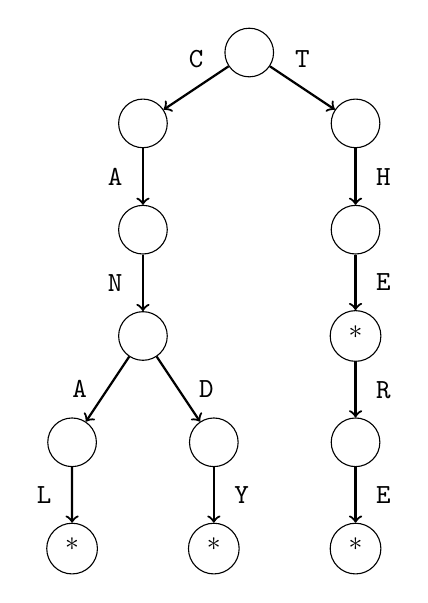
\begin{tikzpicture}[scale=0.9]
\node[draw, circle] (1) at (0,20) {$\phantom{1}$};
\node[draw, circle] (2) at (-1.5,19) {$\phantom{1}$};
\node[draw, circle] (3) at (1.5,19) {$\phantom{1}$};
\node[draw, circle] (4) at (-1.5,17.5) {$\phantom{1}$};
\node[draw, circle] (5) at (-1.5,16) {$\phantom{1}$};
\node[draw, circle] (6) at (-2.5,14.5) {$\phantom{1}$};
\node[draw, circle] (7) at (-0.5,14.5) {$\phantom{1}$};
\node[draw, circle] (8) at (-2.5,13) {*};
\node[draw, circle] (9) at (-0.5,13) {*};
\node[draw, circle] (10) at (1.5,17.5) {$\phantom{1}$};
\node[draw, circle] (11) at (1.5,16) {*};
\node[draw, circle] (12) at (1.5,14.5) {$\phantom{1}$};
\node[draw, circle] (13) at (1.5,13) {*};

\path[draw,thick,->] (1) -- node[font=\small,label=\texttt{C}] {} (2);
\path[draw,thick,->] (1) -- node[font=\small,label=\texttt{T}] {} (3);
\path[draw,thick,->] (2) -- node[font=\small,label=left:\texttt{A}] {} (4);
\path[draw,thick,->] (4) -- node[font=\small,label=left:\texttt{N}] {} (5);
\path[draw,thick,->] (5) -- node[font=\small,label=left:\texttt{A}] {} (6);
\path[draw,thick,->] (5) -- node[font=\small,label=right:\texttt{D}] {} (7);
\path[draw,thick,->] (6) -- node[font=\small,label=left:\texttt{L}] {}(8);
\path[draw,thick,->] (7) -- node[font=\small,label=right:\texttt{Y}] {} (9);
\path[draw,thick,->] (3) -- node[font=\small,label=right:\texttt{H}] {} (10);
\path[draw,thick,->] (10) -- node[font=\small,label=right:\texttt{E}] {} (11);
\path[draw,thick,->] (11) -- node[font=\small,label=right:\texttt{R}] {} (12);
\path[draw,thick,->] (12) -- node[font=\small,label=right:\texttt{E}] {} (13);
\end{tikzpicture}
\end{center}

这个Trie对应于集合
$\{\texttt{CANAL},\texttt{CANDY},\texttt{THE},\texttt{THERE}\}$。
节点中的字符 * 表示集合中的一个字符串
在该节点处结束。
需要这样的字符，因为一个字符串
可能是另一个字符串的前缀。
例如，在上面的Trie中，\texttt{THE}
是 \texttt{THERE} 的前缀。

我们可以在 $O(n)$ 时间内检查Trie
是否包含长度为 $n$ 的字符串，
因为我们可以沿着从根节点开始的链进行跟踪。
我们也可以在 $O(n)$ 时间内向Trie中
添加一个长度为 $n$ 的字符串，
方法是先沿着链跟踪，
然后在必要时向Trie中添加新节点。

使用Trie，我们可以找到
给定字符串的最长前缀，
使得该前缀属于集合。
此外，通过在每个节点中存储额外信息，
我们可以计算集合中以给定字符串
作为前缀的字符串数量。

Trie可以存储在数组中
\begin{lstlisting}
int trie[N][A];
\end{lstlisting}
其中 $N$ 是最大节点数
（集合中字符串的最大总长度），
$A$ 是字母表的大小。
Trie的节点编号为
$0,1,2,\ldots$，根节点的编号为0，
$\texttt{trie}[s][c]$ 是从节点 $s$ 使用字符 $c$
移动时的下一个节点。

\section{字符串哈希}

\index{哈希}
\index{字符串哈希}

\key{字符串哈希}是一种技术，
允许我们高效地检查两个字符串是否相等\footnote{该技术由 Karp–Rabin 模式匹配算法 \cite{kar87} 推广。}。
字符串哈希的思想是比较字符串的哈希值，
而不是逐个比较字符。

\subsubsection*{计算哈希值}

\index{哈希值}
\index{多项式哈希}

字符串的\key{哈希值}是
从字符串的字符计算得出的
一个数字。
如果两个字符串相同，
它们的哈希值也相同，
这使得基于哈希值比较字符串
成为可能。

实现字符串哈希的常用方法是\key{多项式哈希}，即
字符串 \texttt{s} （长度为 $n$）的哈希值为
\[(\texttt{s}[0] A^{n-1} + \texttt{s}[1] A^{n-2} + \cdots + \texttt{s}[n-1] A^0) \bmod B  ,\]
其中 $s[0],s[1],\ldots,s[n-1]$
被解释为 \texttt{s} 各字符的编码，
$A$ 和 $B$ 是预先选定的常数。

例如，\texttt{ALLEY} 各字符的编码为：
\begin{center}
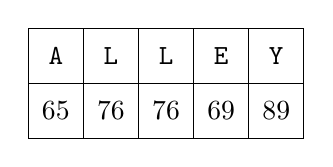
\begin{tikzpicture}[scale=0.7]
\draw (0,0) grid (5,2);

\node at (0.5, 1.5) {\texttt{A}};
\node at (1.5, 1.5) {\texttt{L}};
\node at (2.5, 1.5) {\texttt{L}};
\node at (3.5, 1.5) {\texttt{E}};
\node at (4.5, 1.5) {\texttt{Y}};

\node at (0.5, 0.5) {65};
\node at (1.5, 0.5) {76};
\node at (2.5, 0.5) {76};
\node at (3.5, 0.5) {69};
\node at (4.5, 0.5) {89};

\end{tikzpicture}
\end{center}

因此，如果 $A=3$ 且 $B=97$，\texttt{ALLEY} 的哈希值为
\[(65 \cdot 3^4 + 76 \cdot 3^3 + 76 \cdot 3^2 + 69 \cdot 3^1 + 89 \cdot 3^0) \bmod 97 = 52.\]

\subsubsection*{预处理}

使用多项式哈希，我们可以在 $O(n)$ 时间的预处理后，
在 $O(1)$ 时间内计算字符串 \texttt{s} 的任意子串的哈希值。
思想是构造数组 \texttt{h}，使得
$\texttt{h}[k]$ 包含前缀 $\texttt{s}[0 \ldots k]$ 的哈希值。
数组值可以递归地计算如下：
\[
\begin{array}{lcl}
\texttt{h}[0] & = & \texttt{s}[0] \\
\texttt{h}[k] & = & (\texttt{h}[k-1] A + \texttt{s}[k]) \bmod B \\
\end{array}
\]
此外，我们构造数组 $\texttt{p}$，
其中 $\texttt{p}[k]=A^k \bmod B$：
\[
\begin{array}{lcl}
\texttt{p}[0] & = & 1 \\
\texttt{p}[k] & = & (\texttt{p}[k-1] A) \bmod B. \\
\end{array}
\]
构造这些数组需要 $O(n)$ 时间。
之后，可以使用公式
\[(\texttt{h}[b]-\texttt{h}[a-1] \texttt{p}[b-a+1]) \bmod B\]
在 $O(1)$ 时间内计算任意子串
$\texttt{s}[a \ldots b]$
的哈希值，
假设 $a>0$。
如果 $a=0$，哈希值就是 $\texttt{h}[b]$。

\subsubsection*{使用哈希值}

我们可以使用哈希值高效地比较字符串。
与其逐个比较字符串的字符，
不如比较它们的哈希值。
如果哈希值相等，
则字符串\emph{很可能}相等，
如果哈希值不同，
则字符串\emph{一定}不同。

使用哈希，我们通常可以使暴力
算法变得高效。
例如，考虑模式匹配问题：
给定字符串 $s$ 和模式 $p$，
找出 $p$ 在 $s$ 中出现的位置。
暴力算法遍历 $p$ 可能出现的所有位置，
并逐个字符比较字符串。
这种算法的时间复杂度为 $O(n^2)$。

我们可以通过使用哈希使暴力算法更高效，
因为算法比较的是字符串的子串。
使用哈希，每次比较只需 $O(1)$ 时间，
因为只比较子串的哈希值。
这产生了一个时间复杂度为 $O(n)$ 的算法，
这也是该问题可能达到的最佳时间复杂度。

通过将哈希与\emph{二分查找}结合，
还可以在对数时间内确定两个字符串的字典序。
这可以通过使用二分查找计算
字符串的公共前缀长度来完成。
一旦知道了公共前缀的长度，
我们只需检查前缀后的下一个字符，
因为这决定了字符串的顺序。

\subsubsection*{冲突与参数}

\index{冲突}

比较哈希值时的一个明显风险是\key{冲突}，即两个字符串
内容不同但哈希值相等。
在这种情况下，依赖哈希值的算法
会得出字符串相等的结论，
但实际上并非如此，
算法可能给出错误的结果。

冲突总是可能的，
因为不同字符串的数量
大于不同哈希值的数量。
然而，如果常数 $A$ 和 $B$ 经过仔细选择，
冲突的概率是很小的。
一种常用的方法是选择接近 $10^9$ 的随机常数，
例如：
\[
\begin{array}{lcl}
A & = & 911382323 \\
B & = & 972663749 \\
\end{array}
\]

使用这样的常数，
可以在计算哈希值时使用
\texttt{long long} 类型，
因为乘积 $AB$ 和 $BB$ 会存入 \texttt{long long}。
但大约 $10^9$ 个不同的哈希值是否足够呢？

让我们考虑三种可以使用哈希的场景：

\textit{场景 1：}字符串 $x$ 和 $y$ 互相比较。
假设所有哈希值等概率出现，
冲突的概率为 $1/B$。

\textit{场景 2：}字符串 $x$ 与字符串
$y_1,y_2,\ldots,y_n$ 比较。
发生一次或多次冲突的概率为

\[1-(1-\frac{1}{B})^n.\]

\textit{场景 3：}所有字符串对 $x_1,x_2,\ldots,x_n$
互相比较。
发生一次或多次冲突的概率为
\[ 1 - \frac{B \cdot (B-1) \cdot (B-2) \cdots (B-n+1)}{B^n}.\]

下表显示了当 $n=10^6$ 且 $B$ 取不同值时的冲突概率：

\begin{center}
\begin{tabular}{rrrr}
常数 $B$ & 场景 1 & 场景 2 & 场景 3 \\
\hline
$10^3$ & $0.001000$ & $1.000000$ & $1.000000$ \\
$10^6$ & $0.000001$ & $0.632121$ & $1.000000$ \\
$10^9$ & $0.000000$ & $0.001000$ & $1.000000$ \\
$10^{12}$ & $0.000000$ & $0.000000$ & $0.393469$ \\
$10^{15}$ & $0.000000$ & $0.000000$ & $0.000500$ \\
$10^{18}$ & $0.000000$ & $0.000000$ & $0.000001$ \\
\end{tabular}
\end{center}

表中显示，在场景 1 中，
当 $B \approx 10^9$ 时，冲突的概率可以忽略不计。
在场景 2 中，冲突是可能的，但概率仍然很小。
然而，在场景 3 中情况非常不同：
当 $B \approx 10^9$ 时，几乎总会发生冲突。

\index{生日悖论}

场景 3 中的现象被称为\key{生日悖论}：
如果一个房间里有 $n$ 个人，
即使 $n$ 很小，\emph{某}两个人
生日相同的概率也很大。
在哈希中，类似地，当所有哈希值互相比较时，
某两个哈希值相等的概率也很大。

我们可以通过使用不同参数计算\emph{多个}哈希值
来降低冲突的概率。
不太可能在所有哈希值中同时发生冲突。
例如，两个参数为 $B \approx 10^9$ 的哈希值
对应于一个参数为 $B \approx 10^{18}$ 的哈希值，
这使得冲突的概率非常小。

有些人使用常数 $B=2^{32}$ 和 $B=2^{64}$，
这很方便，因为 32 位和 64 位整数的运算
是模 $2^{32}$ 和 $2^{64}$ 计算的。
然而，这\emph{并不}是一个好的选择，因为可以构造出
在使用 $2^x$ 形式的常数时总是产生冲突的输入 \cite{pac13}。

\section{Z算法}

\index{Z算法}
\index{Z数组}

字符串 \texttt{s} （长度为 $n$）的\key{Z数组} \texttt{z}
对于每个 $k=0,1,\ldots,n-1$ 包含
\texttt{s} 中从位置 $k$ 开始且是 \texttt{s} 的前缀的
最长子串的长度。
因此，$\texttt{z}[k]=p$ 告诉我们
$\texttt{s}[0 \ldots p-1]$ 等于 $\texttt{s}[k \ldots k+p-1]$。
许多字符串处理问题可以使用Z数组高效解决。

例如，\texttt{ACBACDACBACBACDA} 的Z数组如下：

\begin{center}
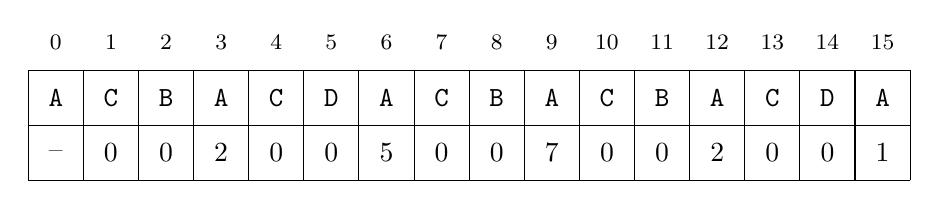
\begin{tikzpicture}[scale=0.7]
\draw (0,0) grid (16,2);

\node at (0.5, 1.5) {\texttt{A}};
\node at (1.5, 1.5) {\texttt{C}};
\node at (2.5, 1.5) {\texttt{B}};
\node at (3.5, 1.5) {\texttt{A}};
\node at (4.5, 1.5) {\texttt{C}};
\node at (5.5, 1.5) {\texttt{D}};
\node at (6.5, 1.5) {\texttt{A}};
\node at (7.5, 1.5) {\texttt{C}};
\node at (8.5, 1.5) {\texttt{B}};
\node at (9.5, 1.5) {\texttt{A}};
\node at (10.5, 1.5) {\texttt{C}};
\node at (11.5, 1.5) {\texttt{B}};
\node at (12.5, 1.5) {\texttt{A}};
\node at (13.5, 1.5) {\texttt{C}};
\node at (14.5, 1.5) {\texttt{D}};
\node at (15.5, 1.5) {\texttt{A}};

\node at (0.5, 0.5) {--};
\node at (1.5, 0.5) {0};
\node at (2.5, 0.5) {0};
\node at (3.5, 0.5) {2};
\node at (4.5, 0.5) {0};
\node at (5.5, 0.5) {0};
\node at (6.5, 0.5) {5};
\node at (7.5, 0.5) {0};
\node at (8.5, 0.5) {0};
\node at (9.5, 0.5) {7};
\node at (10.5, 0.5) {0};
\node at (11.5, 0.5) {0};
\node at (12.5, 0.5) {2};
\node at (13.5, 0.5) {0};
\node at (14.5, 0.5) {0};
\node at (15.5, 0.5) {1};

\footnotesize
\node at (0.5, 2.5) {0};
\node at (1.5, 2.5) {1};
\node at (2.5, 2.5) {2};
\node at (3.5, 2.5) {3};
\node at (4.5, 2.5) {4};
\node at (5.5, 2.5) {5};
\node at (6.5, 2.5) {6};
\node at (7.5, 2.5) {7};
\node at (8.5, 2.5) {8};
\node at (9.5, 2.5) {9};
\node at (10.5, 2.5) {10};
\node at (11.5, 2.5) {11};
\node at (12.5, 2.5) {12};
\node at (13.5, 2.5) {13};
\node at (14.5, 2.5) {14};
\node at (15.5, 2.5) {15};

\end{tikzpicture}
\end{center}

例如，在这个例子中，$\texttt{z}[6]=5$，
因为长度为 5 的子串 \texttt{ACBAC}
是 \texttt{s} 的前缀，
但长度为 6 的子串 \texttt{ACBACB}
不是 \texttt{s} 的前缀。

\subsubsection*{算法描述}

接下来我们描述一个算法，
称为\key{Z算法}\footnote{Z算法在 \cite{gus97} 中作为线性时间模式匹配的最简已知方法被提出，原始思想归功于 \cite{mai84}。}，
它可以在 $O(n)$ 时间内高效构造Z数组。
该算法从左到右计算Z数组的值，
既使用Z数组中已存储的信息，
也逐个字符比较子串。

为了高效计算Z数组的值，
算法维护一个区间 $[x,y]$，
使得 $\texttt{s}[x \ldots y]$ 是 \texttt{s} 的前缀
且 $y$ 尽可能大。
由于我们知道 $\texttt{s}[0 \ldots y-x]$
和 $\texttt{s}[x \ldots y]$ 相等，
我们可以在计算位置 $x+1,x+2,\ldots,y$ 的Z值时
利用这一信息。

在每个位置 $k$，我们首先
检查 $\texttt{z}[k-x]$ 的值。
如果 $k+\texttt{z}[k-x]<y$，我们知道 $\texttt{z}[k]=\texttt{z}[k-x]$。
然而，如果 $k+\texttt{z}[k-x] \ge y$，
$\texttt{s}[0 \ldots y-k]$ 等于
$\texttt{s}[k \ldots y]$，为了确定
$\texttt{z}[k]$ 的值，我们需要
逐个字符比较子串。
尽管如此，算法仍在 $O(n)$ 时间内工作，
因为我们从位置 $y-k+1$ 和 $y+1$
开始比较。

例如，让我们构造以下Z数组：

\begin{center}
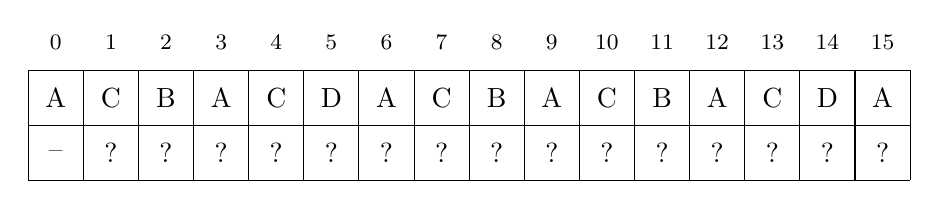
\begin{tikzpicture}[scale=0.7]
\draw (0,0) grid (16,2);

\node at (0.5, 1.5) {A};
\node at (1.5, 1.5) {C};
\node at (2.5, 1.5) {B};
\node at (3.5, 1.5) {A};
\node at (4.5, 1.5) {C};
\node at (5.5, 1.5) {D};
\node at (6.5, 1.5) {A};
\node at (7.5, 1.5) {C};
\node at (8.5, 1.5) {B};
\node at (9.5, 1.5) {A};
\node at (10.5, 1.5) {C};
\node at (11.5, 1.5) {B};
\node at (12.5, 1.5) {A};
\node at (13.5, 1.5) {C};
\node at (14.5, 1.5) {D};
\node at (15.5, 1.5) {A};

\node at (0.5, 0.5) {--};
\node at (1.5, 0.5) {?};
\node at (2.5, 0.5) {?};
\node at (3.5, 0.5) {?};
\node at (4.5, 0.5) {?};
\node at (5.5, 0.5) {?};
\node at (6.5, 0.5) {?};
\node at (7.5, 0.5) {?};
\node at (8.5, 0.5) {?};
\node at (9.5, 0.5) {?};
\node at (10.5, 0.5) {?};
\node at (11.5, 0.5) {?};
\node at (12.5, 0.5) {?};
\node at (13.5, 0.5) {?};
\node at (14.5, 0.5) {?};
\node at (15.5, 0.5) {?};

\footnotesize
\node at (0.5, 2.5) {0};
\node at (1.5, 2.5) {1};
\node at (2.5, 2.5) {2};
\node at (3.5, 2.5) {3};
\node at (4.5, 2.5) {4};
\node at (5.5, 2.5) {5};
\node at (6.5, 2.5) {6};
\node at (7.5, 2.5) {7};
\node at (8.5, 2.5) {8};
\node at (9.5, 2.5) {9};
\node at (10.5, 2.5) {10};
\node at (11.5, 2.5) {11};
\node at (12.5, 2.5) {12};
\node at (13.5, 2.5) {13};
\node at (14.5, 2.5) {14};
\node at (15.5, 2.5) {15};

\end{tikzpicture}
\end{center}

在计算值 $\texttt{z}[6]=5$ 后，
当前的 $[x,y]$ 区间是 $[6,10]$：

\begin{center}
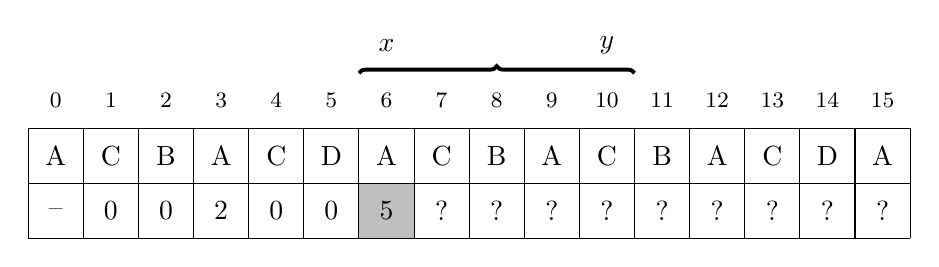
\begin{tikzpicture}[scale=0.7]
\fill[color=lightgray] (6,0) rectangle (7,1);
\draw (0,0) grid (16,2);

\node at (0.5, 1.5) {A};
\node at (1.5, 1.5) {C};
\node at (2.5, 1.5) {B};
\node at (3.5, 1.5) {A};
\node at (4.5, 1.5) {C};
\node at (5.5, 1.5) {D};
\node at (6.5, 1.5) {A};
\node at (7.5, 1.5) {C};
\node at (8.5, 1.5) {B};
\node at (9.5, 1.5) {A};
\node at (10.5, 1.5) {C};
\node at (11.5, 1.5) {B};
\node at (12.5, 1.5) {A};
\node at (13.5, 1.5) {C};
\node at (14.5, 1.5) {D};
\node at (15.5, 1.5) {A};

\node at (0.5, 0.5) {--};
\node at (1.5, 0.5) {0};
\node at (2.5, 0.5) {0};
\node at (3.5, 0.5) {2};
\node at (4.5, 0.5) {0};
\node at (5.5, 0.5) {0};
\node at (6.5, 0.5) {5};
\node at (7.5, 0.5) {?};
\node at (8.5, 0.5) {?};
\node at (9.5, 0.5) {?};
\node at (10.5, 0.5) {?};
\node at (11.5, 0.5) {?};
\node at (12.5, 0.5) {?};
\node at (13.5, 0.5) {?};
\node at (14.5, 0.5) {?};
\node at (15.5, 0.5) {?};

\draw [decoration={brace}, decorate, line width=0.5mm] (6,3.00) -- (11,3.00);

\node at (6.5,3.50) {$x$};
\node at (10.5,3.50) {$y$};


\footnotesize
\node at (0.5, 2.5) {0};
\node at (1.5, 2.5) {1};
\node at (2.5, 2.5) {2};
\node at (3.5, 2.5) {3};
\node at (4.5, 2.5) {4};
\node at (5.5, 2.5) {5};
\node at (6.5, 2.5) {6};
\node at (7.5, 2.5) {7};
\node at (8.5, 2.5) {8};
\node at (9.5, 2.5) {9};
\node at (10.5, 2.5) {10};
\node at (11.5, 2.5) {11};
\node at (12.5, 2.5) {12};
\node at (13.5, 2.5) {13};
\node at (14.5, 2.5) {14};
\node at (15.5, 2.5) {15};

\end{tikzpicture}
\end{center}

现在我们可以高效地计算
后续的Z数组值，
因为我们知道
$\texttt{s}[0 \ldots 4]$ 和
$\texttt{s}[6 \ldots 10]$ 相等。
首先，由于 $\texttt{z}[1] = \texttt{z}[2] = 0$，
我们立即可知
$\texttt{z}[7] = \texttt{z}[8] = 0$：

\begin{center}
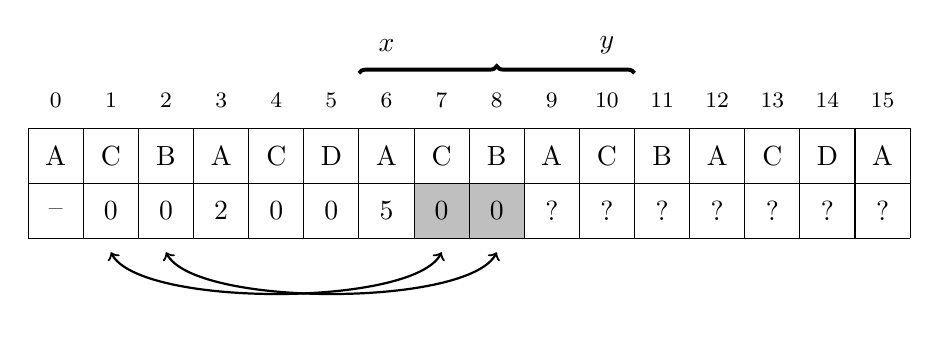
\begin{tikzpicture}[scale=0.7]
\fill[color=lightgray] (7,0) rectangle (9,1);
\draw (0,0) grid (16,2);

\node at (0.5, 1.5) {A};
\node at (1.5, 1.5) {C};
\node at (2.5, 1.5) {B};
\node at (3.5, 1.5) {A};
\node at (4.5, 1.5) {C};
\node at (5.5, 1.5) {D};
\node at (6.5, 1.5) {A};
\node at (7.5, 1.5) {C};
\node at (8.5, 1.5) {B};
\node at (9.5, 1.5) {A};
\node at (10.5, 1.5) {C};
\node at (11.5, 1.5) {B};
\node at (12.5, 1.5) {A};
\node at (13.5, 1.5) {C};
\node at (14.5, 1.5) {D};
\node at (15.5, 1.5) {A};

\node at (0.5, 0.5) {--};
\node at (1.5, 0.5) {0};
\node at (2.5, 0.5) {0};
\node at (3.5, 0.5) {2};
\node at (4.5, 0.5) {0};
\node at (5.5, 0.5) {0};
\node at (6.5, 0.5) {5};
\node at (7.5, 0.5) {0};
\node at (8.5, 0.5) {0};
\node at (9.5, 0.5) {?};
\node at (10.5, 0.5) {?};
\node at (11.5, 0.5) {?};
\node at (12.5, 0.5) {?};
\node at (13.5, 0.5) {?};
\node at (14.5, 0.5) {?};
\node at (15.5, 0.5) {?};


\draw [decoration={brace}, decorate, line width=0.5mm] (6,3.00) -- (11,3.00);

\node at (6.5,3.50) {$x$};
\node at (10.5,3.50) {$y$};


\footnotesize
\node at (0.5, 2.5) {0};
\node at (1.5, 2.5) {1};
\node at (2.5, 2.5) {2};
\node at (3.5, 2.5) {3};
\node at (4.5, 2.5) {4};
\node at (5.5, 2.5) {5};
\node at (6.5, 2.5) {6};
\node at (7.5, 2.5) {7};
\node at (8.5, 2.5) {8};
\node at (9.5, 2.5) {9};
\node at (10.5, 2.5) {10};
\node at (11.5, 2.5) {11};
\node at (12.5, 2.5) {12};
\node at (13.5, 2.5) {13};
\node at (14.5, 2.5) {14};
\node at (15.5, 2.5) {15};


\draw[thick,<->] (7.5,-0.25) .. controls (7,-1.25) and (2,-1.25) .. (1.5,-0.25);
\draw[thick,<->] (8.5,-0.25) .. controls (8,-1.25) and (3,-1.25) .. (2.5,-0.25);
\end{tikzpicture}
\end{center}

然后，由于 $\texttt{z}[3]=2$，我们知道 $\texttt{z}[9] \ge 2$：

\begin{center}
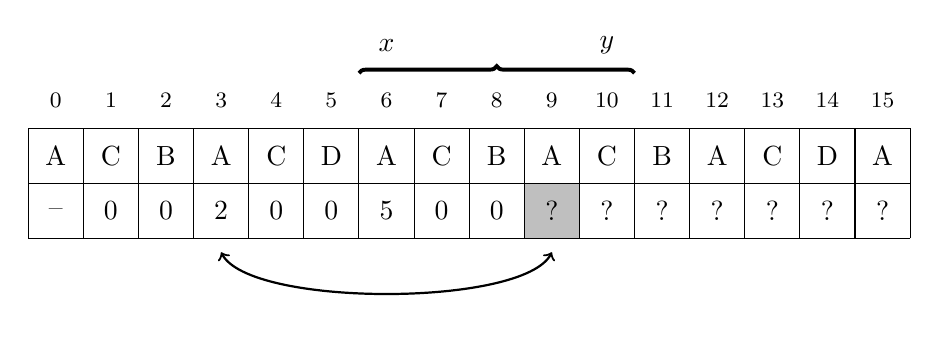
\begin{tikzpicture}[scale=0.7]
\fill[color=lightgray] (9,0) rectangle (10,1);
\draw (0,0) grid (16,2);

\node at (0.5, 1.5) {A};
\node at (1.5, 1.5) {C};
\node at (2.5, 1.5) {B};
\node at (3.5, 1.5) {A};
\node at (4.5, 1.5) {C};
\node at (5.5, 1.5) {D};
\node at (6.5, 1.5) {A};
\node at (7.5, 1.5) {C};
\node at (8.5, 1.5) {B};
\node at (9.5, 1.5) {A};
\node at (10.5, 1.5) {C};
\node at (11.5, 1.5) {B};
\node at (12.5, 1.5) {A};
\node at (13.5, 1.5) {C};
\node at (14.5, 1.5) {D};
\node at (15.5, 1.5) {A};

\node at (0.5, 0.5) {--};
\node at (1.5, 0.5) {0};
\node at (2.5, 0.5) {0};
\node at (3.5, 0.5) {2};
\node at (4.5, 0.5) {0};
\node at (5.5, 0.5) {0};
\node at (6.5, 0.5) {5};
\node at (7.5, 0.5) {0};
\node at (8.5, 0.5) {0};
\node at (9.5, 0.5) {?};
\node at (10.5, 0.5) {?};
\node at (11.5, 0.5) {?};
\node at (12.5, 0.5) {?};
\node at (13.5, 0.5) {?};
\node at (14.5, 0.5) {?};
\node at (15.5, 0.5) {?};

\draw [decoration={brace}, decorate, line width=0.5mm] (6,3.00) -- (11,3.00);

\node at (6.5,3.50) {$x$};
\node at (10.5,3.50) {$y$};


\footnotesize
\node at (0.5, 2.5) {0};
\node at (1.5, 2.5) {1};
\node at (2.5, 2.5) {2};
\node at (3.5, 2.5) {3};
\node at (4.5, 2.5) {4};
\node at (5.5, 2.5) {5};
\node at (6.5, 2.5) {6};
\node at (7.5, 2.5) {7};
\node at (8.5, 2.5) {8};
\node at (9.5, 2.5) {9};
\node at (10.5, 2.5) {10};
\node at (11.5, 2.5) {11};
\node at (12.5, 2.5) {12};
\node at (13.5, 2.5) {13};
\node at (14.5, 2.5) {14};
\node at (15.5, 2.5) {15};

\draw[thick,<->] (9.5,-0.25) .. controls (9,-1.25) and (4,-1.25) .. (3.5,-0.25);
\end{tikzpicture}
\end{center}

然而，我们没有关于位置 10 之后字符串的信息，
因此需要逐个字符比较子串：

\begin{center}
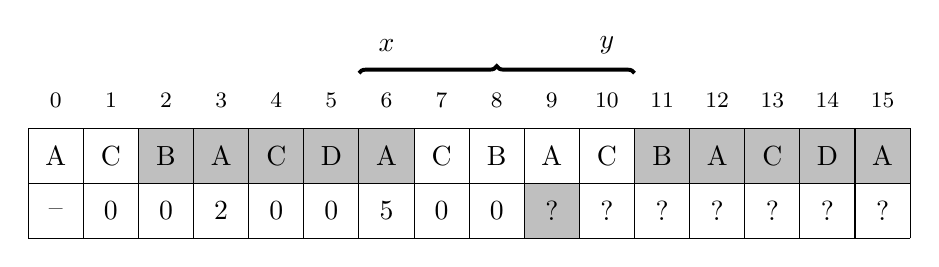
\begin{tikzpicture}[scale=0.7]
\fill[color=lightgray] (9,0) rectangle (10,1);
\fill[color=lightgray] (2,1) rectangle (7,2);
\fill[color=lightgray] (11,1) rectangle (16,2);


\draw (0,0) grid (16,2);

\node at (0.5, 1.5) {A};
\node at (1.5, 1.5) {C};
\node at (2.5, 1.5) {B};
\node at (3.5, 1.5) {A};
\node at (4.5, 1.5) {C};
\node at (5.5, 1.5) {D};
\node at (6.5, 1.5) {A};
\node at (7.5, 1.5) {C};
\node at (8.5, 1.5) {B};
\node at (9.5, 1.5) {A};
\node at (10.5, 1.5) {C};
\node at (11.5, 1.5) {B};
\node at (12.5, 1.5) {A};
\node at (13.5, 1.5) {C};
\node at (14.5, 1.5) {D};
\node at (15.5, 1.5) {A};

\node at (0.5, 0.5) {--};
\node at (1.5, 0.5) {0};
\node at (2.5, 0.5) {0};
\node at (3.5, 0.5) {2};
\node at (4.5, 0.5) {0};
\node at (5.5, 0.5) {0};
\node at (6.5, 0.5) {5};
\node at (7.5, 0.5) {0};
\node at (8.5, 0.5) {0};
\node at (9.5, 0.5) {?};
\node at (10.5, 0.5) {?};
\node at (11.5, 0.5) {?};
\node at (12.5, 0.5) {?};
\node at (13.5, 0.5) {?};
\node at (14.5, 0.5) {?};
\node at (15.5, 0.5) {?};

\draw [decoration={brace}, decorate, line width=0.5mm] (6,3.00) -- (11,3.00);

\node at (6.5,3.50) {$x$};
\node at (10.5,3.50) {$y$};


\footnotesize
\node at (0.5, 2.5) {0};
\node at (1.5, 2.5) {1};
\node at (2.5, 2.5) {2};
\node at (3.5, 2.5) {3};
\node at (4.5, 2.5) {4};
\node at (5.5, 2.5) {5};
\node at (6.5, 2.5) {6};
\node at (7.5, 2.5) {7};
\node at (8.5, 2.5) {8};
\node at (9.5, 2.5) {9};
\node at (10.5, 2.5) {10};
\node at (11.5, 2.5) {11};
\node at (12.5, 2.5) {12};
\node at (13.5, 2.5) {13};
\node at (14.5, 2.5) {14};
\node at (15.5, 2.5) {15};

%\draw[thick,<->] (11.5,-0.25) .. controls (11,-1.25) and (3,-1.25) .. (2.5,-0.25);
\end{tikzpicture}
\end{center}

结果是 $\texttt{z}[9]=7$，
所以新的 $[x,y]$ 区间是 $[9,15]$：

\begin{center}
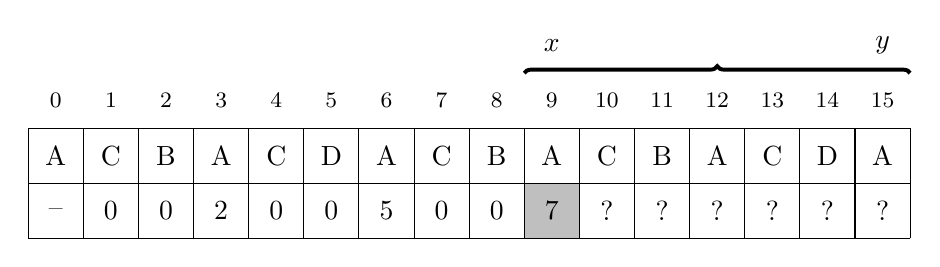
\begin{tikzpicture}[scale=0.7]
\fill[color=lightgray] (9,0) rectangle (10,1);
\draw (0,0) grid (16,2);

\node at (0.5, 1.5) {A};
\node at (1.5, 1.5) {C};
\node at (2.5, 1.5) {B};
\node at (3.5, 1.5) {A};
\node at (4.5, 1.5) {C};
\node at (5.5, 1.5) {D};
\node at (6.5, 1.5) {A};
\node at (7.5, 1.5) {C};
\node at (8.5, 1.5) {B};
\node at (9.5, 1.5) {A};
\node at (10.5, 1.5) {C};
\node at (11.5, 1.5) {B};
\node at (12.5, 1.5) {A};
\node at (13.5, 1.5) {C};
\node at (14.5, 1.5) {D};
\node at (15.5, 1.5) {A};

\node at (0.5, 0.5) {--};
\node at (1.5, 0.5) {0};
\node at (2.5, 0.5) {0};
\node at (3.5, 0.5) {2};
\node at (4.5, 0.5) {0};
\node at (5.5, 0.5) {0};
\node at (6.5, 0.5) {5};
\node at (7.5, 0.5) {0};
\node at (8.5, 0.5) {0};
\node at (9.5, 0.5) {7};
\node at (10.5, 0.5) {?};
\node at (11.5, 0.5) {?};
\node at (12.5, 0.5) {?};
\node at (13.5, 0.5) {?};
\node at (14.5, 0.5) {?};
\node at (15.5, 0.5) {?};

\draw [decoration={brace}, decorate, line width=0.5mm] (9,3.00) -- (16,3.00);

\node at (9.5,3.50) {$x$};
\node at (15.5,3.50) {$y$};


\footnotesize
\node at (0.5, 2.5) {0};
\node at (1.5, 2.5) {1};
\node at (2.5, 2.5) {2};
\node at (3.5, 2.5) {3};
\node at (4.5, 2.5) {4};
\node at (5.5, 2.5) {5};
\node at (6.5, 2.5) {6};
\node at (7.5, 2.5) {7};
\node at (8.5, 2.5) {8};
\node at (9.5, 2.5) {9};
\node at (10.5, 2.5) {10};
\node at (11.5, 2.5) {11};
\node at (12.5, 2.5) {12};
\node at (13.5, 2.5) {13};
\node at (14.5, 2.5) {14};
\node at (15.5, 2.5) {15};

% \draw[thick,<->] (9.5,-0.25) .. controls (9,-1.25) and (4,-1.25) .. (3.5,-0.25);
\end{tikzpicture}
\end{center}

此后，所有剩余的Z数组值
都可以利用Z数组中已存储的
信息来确定：

\begin{center}
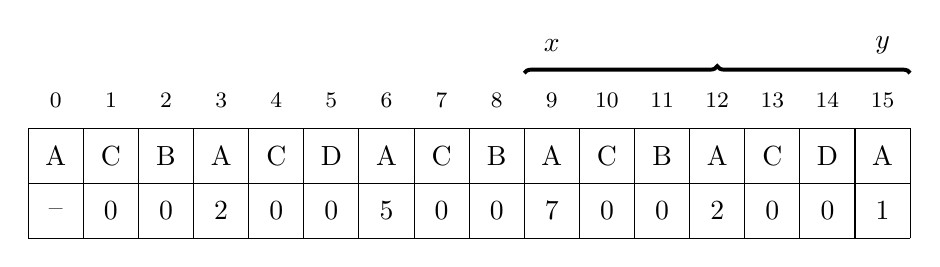
\begin{tikzpicture}[scale=0.7]
\draw (0,0) grid (16,2);

\node at (0.5, 1.5) {A};
\node at (1.5, 1.5) {C};
\node at (2.5, 1.5) {B};
\node at (3.5, 1.5) {A};
\node at (4.5, 1.5) {C};
\node at (5.5, 1.5) {D};
\node at (6.5, 1.5) {A};
\node at (7.5, 1.5) {C};
\node at (8.5, 1.5) {B};
\node at (9.5, 1.5) {A};
\node at (10.5, 1.5) {C};
\node at (11.5, 1.5) {B};
\node at (12.5, 1.5) {A};
\node at (13.5, 1.5) {C};
\node at (14.5, 1.5) {D};
\node at (15.5, 1.5) {A};

\node at (0.5, 0.5) {--};
\node at (1.5, 0.5) {0};
\node at (2.5, 0.5) {0};
\node at (3.5, 0.5) {2};
\node at (4.5, 0.5) {0};
\node at (5.5, 0.5) {0};
\node at (6.5, 0.5) {5};
\node at (7.5, 0.5) {0};
\node at (8.5, 0.5) {0};
\node at (9.5, 0.5) {7};
\node at (10.5, 0.5) {0};
\node at (11.5, 0.5) {0};
\node at (12.5, 0.5) {2};
\node at (13.5, 0.5) {0};
\node at (14.5, 0.5) {0};
\node at (15.5, 0.5) {1};

\draw [decoration={brace}, decorate, line width=0.5mm] (9,3.00) -- (16,3.00);

\node at (9.5,3.50) {$x$};
\node at (15.5,3.50) {$y$};


\footnotesize
\node at (0.5, 2.5) {0};
\node at (1.5, 2.5) {1};
\node at (2.5, 2.5) {2};
\node at (3.5, 2.5) {3};
\node at (4.5, 2.5) {4};
\node at (5.5, 2.5) {5};
\node at (6.5, 2.5) {6};
\node at (7.5, 2.5) {7};
\node at (8.5, 2.5) {8};
\node at (9.5, 2.5) {9};
\node at (10.5, 2.5) {10};
\node at (11.5, 2.5) {11};
\node at (12.5, 2.5) {12};
\node at (13.5, 2.5) {13};
\node at (14.5, 2.5) {14};
\node at (15.5, 2.5) {15};

\end{tikzpicture}
\end{center}

\subsubsection{使用Z数组}

使用字符串哈希还是Z算法通常取决于个人偏好。
与哈希不同，Z算法总是有效，
且没有冲突的风险。
另一方面，Z算法实现起来更困难，
而且某些问题只能使用哈希来解决。

例如，再次考虑模式匹配问题，
我们的任务是找出模式 $p$ 在字符串 $s$ 中出现的位置。
我们已经使用字符串哈希高效地解决了这个问题，
但Z算法提供了另一种解决问题的方法。

字符串处理中的一种常用思想是
构造一个由多个字符串通过特殊字符分隔组成的字符串。
在这个问题中，我们可以构造字符串
$p$\texttt{\#}$s$，
其中 $p$ 和 $s$ 由一个不出现在
字符串中的特殊字符 \texttt{\#} 分隔。
$p$\texttt{\#}$s$ 的Z数组告诉我们 $p$ 在 $s$ 中出现的位置，
因为这些位置包含了 $p$ 的长度。

例如，如果 $s=$\texttt{HATTIVATTI} 且 $p=$\texttt{ATT}，
Z数组如下：

\begin{center}
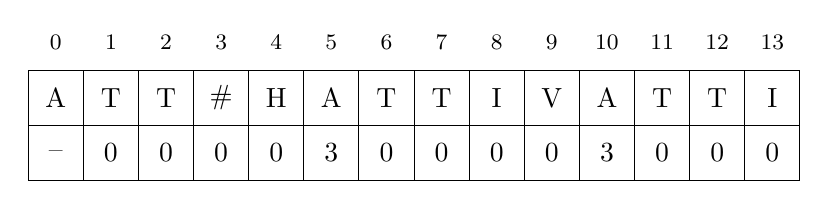
\begin{tikzpicture}[scale=0.7]
\draw (0,0) grid (14,2);

\node at (0.5, 1.5) {A};
\node at (1.5, 1.5) {T};
\node at (2.5, 1.5) {T};
\node at (3.5, 1.5) {\#};
\node at (4.5, 1.5) {H};
\node at (5.5, 1.5) {A};
\node at (6.5, 1.5) {T};
\node at (7.5, 1.5) {T};
\node at (8.5, 1.5) {I};
\node at (9.5, 1.5) {V};
\node at (10.5, 1.5) {A};
\node at (11.5, 1.5) {T};
\node at (12.5, 1.5) {T};
\node at (13.5, 1.5) {I};

\node at (0.5, 0.5) {--};
\node at (1.5, 0.5) {0};
\node at (2.5, 0.5) {0};
\node at (3.5, 0.5) {0};
\node at (4.5, 0.5) {0};
\node at (5.5, 0.5) {3};
\node at (6.5, 0.5) {0};
\node at (7.5, 0.5) {0};
\node at (8.5, 0.5) {0};
\node at (9.5, 0.5) {0};
\node at (10.5, 0.5) {3};
\node at (11.5, 0.5) {0};
\node at (12.5, 0.5) {0};
\node at (13.5, 0.5) {0};

\footnotesize
\node at (0.5, 2.5) {0};
\node at (1.5, 2.5) {1};
\node at (2.5, 2.5) {2};
\node at (3.5, 2.5) {3};
\node at (4.5, 2.5) {4};
\node at (5.5, 2.5) {5};
\node at (6.5, 2.5) {6};
\node at (7.5, 2.5) {7};
\node at (8.5, 2.5) {8};
\node at (9.5, 2.5) {9};
\node at (10.5, 2.5) {10};
\node at (11.5, 2.5) {11};
\node at (12.5, 2.5) {12};
\node at (13.5, 2.5) {13};
\end{tikzpicture}
\end{center}

位置 5 和 10 包含值 3，
这意味着模式 \texttt{ATT}
出现在 \texttt{HATTIVATTI} 的对应位置。

所得算法的时间复杂度是线性的，
因为只需构造Z数组并遍历其值即可。

\subsubsection{实现}

以下是Z算法的一个简短实现，
返回一个对应于Z数组的 vector。

\begin{lstlisting}
vector<int> z(string s) {
    int n = s.size();
    vector<int> z(n);
    int x = 0, y = 0;
    for (int i = 1; i < n; i++) {
        z[i] = max(0,min(z[i-x],y-i+1));
        while (i+z[i] < n && s[z[i]] == s[i+z[i]]) {
            x = i; y = i+z[i]; z[i]++;
        }
    }
    return z;
}
\end{lstlisting}